\subsection{Maximale Drehzahl bei variabler Spannung}\label{subsec:DrehzahlSpanungsabfall}
In diesem Versuch wird das Verhalten des Motors bei Unterspannung untersucht. Dabei wurde der Sollwert für das Drehmoment auf dem Maximum gehalten, während der Motor im Leerlauf dreht. Die Spannung wird dabei langsam erhöht.

\begin{table}[H]
	\centering
	\begin{tabular}{C{4cm} C{4cm} C{3cm}} 
		\multicolumn{3}{c}{\textbf{Versuchsbedingungen}} \\
		{Messgrösse}& {Bedingung} & {Wert}\\ \hline\hline 
		Spannung (DC)   & variiert &   64.7-90.7 V     \\
		Strom (DC)   & gemessen &   9.33-13.1 A     \\
		Leistung (AC)   & vernachlässigt &   -    \\
		Drehzahl   & gemessen &   3600 RPM    \\
		Drehmoment-Sollwert   & konstant &   max.    \\
		Motor-Temperatur   & vernachlässigt &   -    \\
		Controller-Temperatur   & vernachlässigt &   -    \\
	\end{tabular}
	\caption{Versuchsbedingungen max. Drehzahl}\label{tab:maxDrehzahl}
\end{table}

 Die Drehzahl ist dabei elektronisch im Controller auf 3800 RPM begrenzt, da die asynchrone Maschine keine höheren Drehzahlen zulässt und ist in nachfolgender Abbildung \ref{fig:maxDrehzahl} graphisch dargestellt.

\begin{figure}[H]
	\centering
	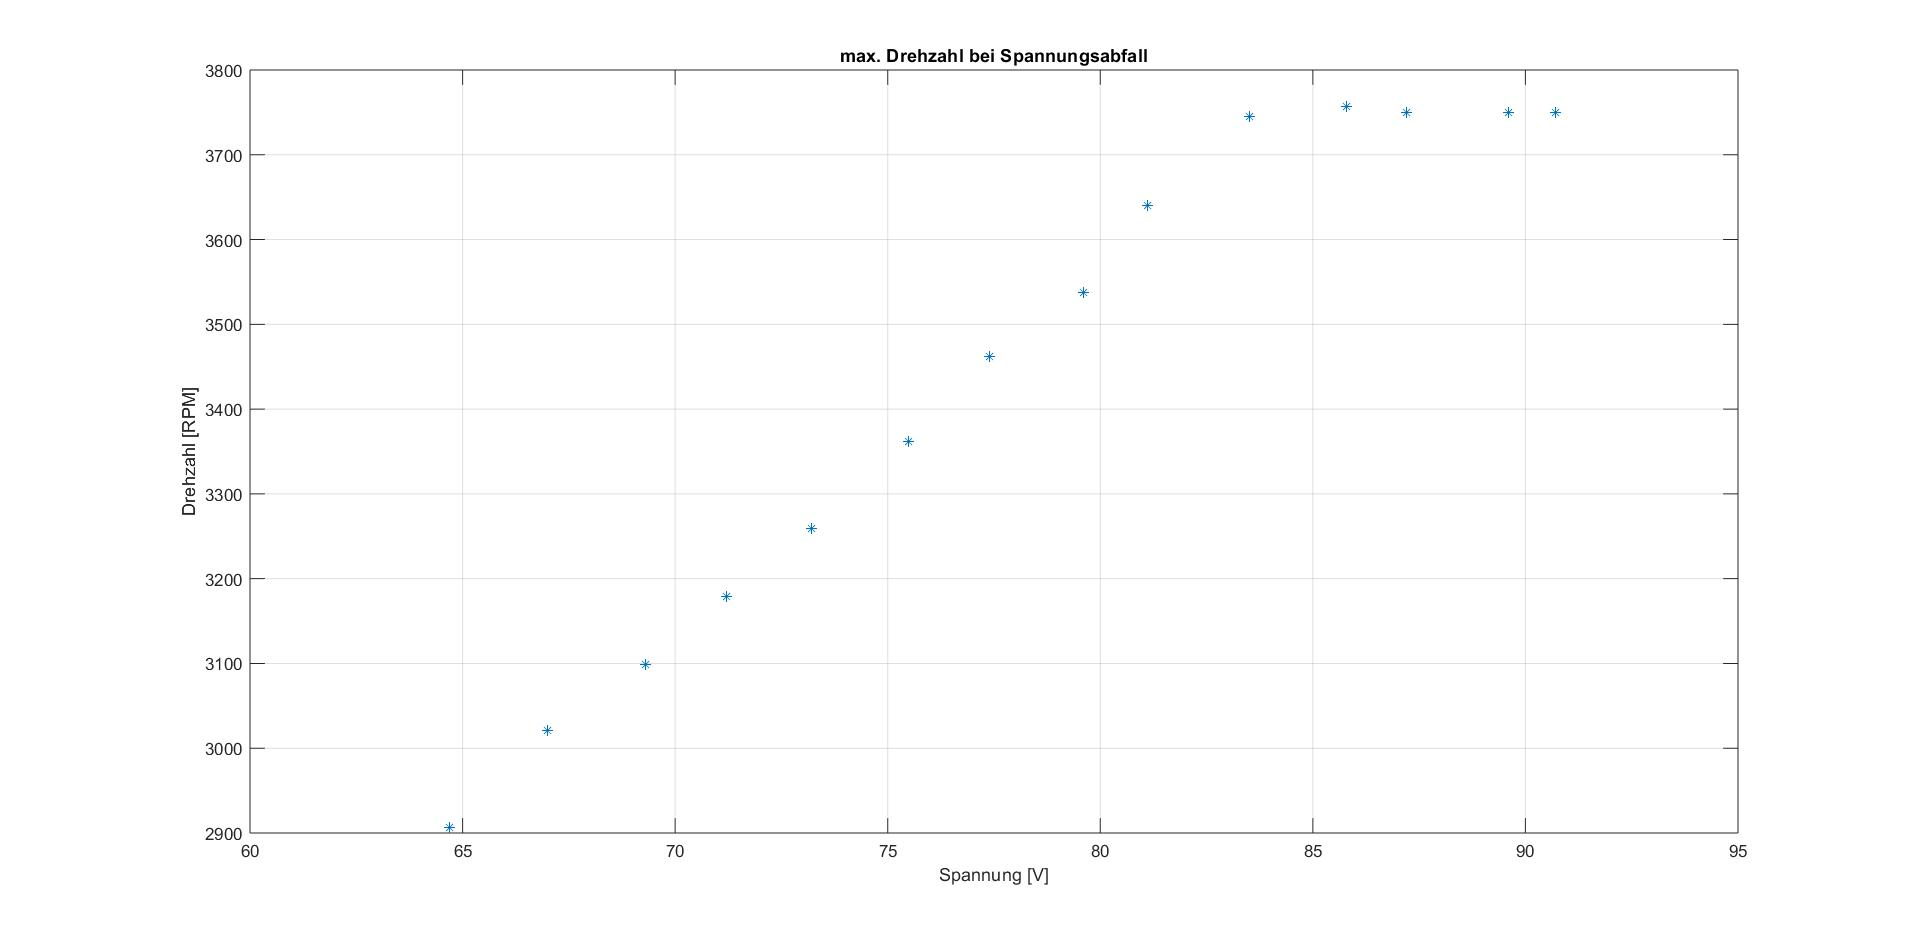
\includegraphics[width=0.8\linewidth]{maxDrehzahl.jpg}
	\caption{Maximale Drehzahl im Leerlauf}\label{fig:maxDrehzahl}
\end{figure}


Bei diesem Versuch hat sich gezeigt, dass die DC-Spannung mindestens 84V betragen muss, damit der BLDC-Motor 3800 RPM erreichen kann. Weiter ist ersichtlich, dass die Leerlaufdrehzahl ca. 45 RPM pro Volt sinkt.
